\documentclass{article}

\usepackage[T1]{fontenc}
\usepackage[french]{babel}

\usepackage[letterpaper,top=2cm,bottom=2cm,left=3cm,right=3cm,marginparwidth=1.75cm]{geometry}

\usepackage{amsmath}
\usepackage{graphicx}
\usepackage[colorlinks=true, allcolors=blue]{hyperref}
\usepackage{eurosym}
\usepackage[group-separator={\ },output-decimal-marker={,}]{siunitx} 
\usepackage{amsfonts}
\usepackage{float}
\usepackage{pdflscape}
\usepackage{algorithm}
\usepackage{algorithmic}
\usepackage{array}
\usepackage{mdframed}
\usepackage{enumitem}
\usepackage{tcolorbox}
\usepackage{fontawesome5} % icônes
\usepackage{xcolor}

\definecolor{lightgreen}{RGB}{230, 255, 230}

\newenvironment{conditions}
  {\par\vspace{\abovedisplayskip}\noindent\begin{tabular}{>{$}l<{$} @{${}={}$} l}}
  {\end{tabular}\par\vspace{\belowdisplayskip}}

\title{Impact de la fréquence de capitalisation sur le taux d'intérêt effectif et la valorisation des investissements}
\author{Gaëtan Bouget}

\begin{document}
\maketitle

\section{Problème}
Dans un contexte financier caractérisé par une diversification accrue des produits d’investissement, la variation des fréquences de capitalisation complique l’évaluation objective des rendements réels. Ainsi, deux actifs affichant un même taux nominal annuel peuvent générer des rendements distincts en raison des différentes fréquences de capitalisation, amplifiant ainsi l'effet des intérêts composés.

\section{Objectif}
L'objectif consiste à fournir une compréhension approfondie des mécanismes influençant le rendement réel des investissements et à établir une base solide pour la comparaison de diverses stratégies financières.

\section{Méthode}
L'approche adoptée pour atteindre l'objectif se décline en quatre étapes :
\begin{enumerate}
    \item calcul du capital final pour les actifs à intérêts simples ;
    \item prise en compte des intérêts composés dans l’analyse comparative ;
    \item démonstration de la supériorité des intérêts composés par développement binomial ;
    \item établissement de la formule du taux effectif annuel (TEA).
\end{enumerate}

Afin de faciliter les applications numériques avant de généraliser, l'analyse se concentre sur l'investissement d'un capital initial de \( C_0 = 100\,000\ \text{€} \), réparti sur quatre actifs décrits dans le tableau~\ref{tab:scenarios}.

\begin{table}[h!]
\centering
\begin{tabular}{|c|c|c|c|}
\hline
\textbf{Actif} & \textbf{Type d'intérêt} & \textbf{Fréquence de capitalisation} & \textbf{Taux périodique} \\
\hline
\(A_q^s\) & Intérêts simples & Quotidienne & \(r_\text{quotidien} = \frac{5}{365}\%\) \\
\hline
\(A_a^s\) & Intérêts simples & Annuelle & \(r_\text{annuel} = 5\%\) \\
\hline
\(A_q^c\) & Intérêts composés & Quotidienne & \(r_\text{quotidien} = \frac{5}{365}\%\) \\
\hline
\(A_a^c\) & Intérêts composés & Annuelle & \(r_\text{annuel} = 5\%\) \\
\hline
\end{tabular}
\caption{Scénarios d'investissement avec un capital initial \(C_0 = 100\,000\ \text{€}\).}
\label{tab:scenarios}
\end{table}

Chaque étape de l'analyse sera ensuite détaillée à travers une série de questions destinées à approfondir la compréhension du phénomène.

\subsection{Hypothèses de travail}
Les conditions suivantes sont posées :
\begin{itemize}
    \item Les intérêts sont calculés selon la fréquence de capitalisation définie pour chaque actif. Aucune capitalisation intermédiaire ni prorata temporis ne s'applique en cas de retrait avant la fin de la période de capitalisation.
    \item Une année est considérée comme comprenant 365 jours.
    \item Aucun frais ni taxe n'est appliqué.
    \item Aucun versement ou retrait supplémentaire n’est effectué durant la période d'investissement (seul le capital initial \( C_0 \) est investi).
    \item Le taux de rendement est constant dans le temps.
    \item L'inflation n'est pas prise en compte.
\end{itemize}

\subsection{Questions}
\subsubsection*{Étape 1 : calcul du capital final pour les actifs à intérêts simples}

\begin{tcolorbox}[
        colback=lightgreen, 
        colframe=lightgreen, 
        boxrule=0.5pt, 
        arc=0pt, 
        left=10pt, 
        right=10pt, 
        top=6pt, 
        bottom=6pt, 
        boxsep=2pt, 
        before upper={\faLightbulb\hspace{10pt}}
    ]
        Les intérêts simples sont calculés uniquement sur le capital initial, et le montant des intérêts gagnés chaque période est constant. La formule suivante reflète bien cette caractéristique, car le produit \( r \times t \) est simplement ajouté au capital initial :

        \[
        C^{\text{simple}}(t) = C_0 \left(1 + r \times t\right)
        \]
        
        où :
        \begin{itemize}
            \item \( C^{\text{simple}}(t) \) est le capital accumulé après une période \( t \).
            \item \( C_0 \) est le capital initial investi.
            \item \( r \) est le taux d'intérêt nominal (exprimé sous forme décimale, par exemple, 5\% devient $\frac{5}{100}$ soit 0,05).
            \item \( t \) est le temps écoulé, qui peut être exprimé en années ou en jours, selon la fréquence de capitalisation.
        \end{itemize}
    \end{tcolorbox}

\begin{enumerate}[label=\textbf{Q\arabic*.}]
    \item Soit un capital initial \( C_0 = 100\,000\ \text{€} \) investi, calculer le capital final de l'actif \( A_q^s \) après une durée \( t \) égale à :
    \begin{enumerate}[label=(\alph*)]
        \item \( t = 1 \) jour
        \item \( t = 30 \) jours
        \item \( t = 1 \) an
        \item \( t = 30 \) ans
    \end{enumerate}

    \item Soit un capital initial \( C_0 = 100\,000\ \text{€} \) investi, calculer le capital final de l'actif \( A_a^s \) après une durée \( t \) égale à :
    \begin{enumerate}[label=(\alph*)]
        \item \( t = 1 \) jour
        \item \( t = 30 \) jours
        \item \( t = 1 \) an
        \item \( t = 30 \) ans
    \end{enumerate}
    
    \item Remplir le tableau suivant en calculant les capitaux finaux pour les deux types d'actifs à différents horizons de temps :\\
    \begin{table}[h!]
        \centering
        \begin{tabular}{|c|c|c|c|c|}
        \hline
        \textbf{Actif} & \textbf{1 jour} & \textbf{30 jours} & \textbf{1 an} & \textbf{30 ans} \\
        \hline
        \( A_q^s \) & & & & \\
        \hline
        \( A_a^s \) & & & & \\
        \hline
        \end{tabular}
        \caption{Capital final pour différentes durées d'investissement avec intérêts simples et un capital initial de \( C_0 = 100\,000\ \text{€} \).}
        \label{tab:simple_interest_results}
    \end{table}

    \item Soit un capital initial \( C_0 \) et un taux nominal annuel \( r_a \) ou un taux nominal quotidien \( r_q \), exprimer les fonctions permettant de calculer le capital final en fonction de la durée d'investissement \( t \) (exprimée en jours) pour chacun des deux actifs à intérêts simples :
    \begin{enumerate}[label=(\alph*)]
        \item \( C^s_q(t) \) pour un actif à capitalisation quotidienne avec un taux périodique \( r_q \) ;
        \item \( C^s_a(t) \) pour un actif à capitalisation annuelle avec un taux \( r_a \).
    \end{enumerate}

    \item Tracer les courbes \( C^s_q(t) \) et \( C^s_a(t) \) pour \( C_0 \in \{50\,000, 100\,000, 200\,000\} \, \text{€} \). La durée \( t \) (en abscisse) varie de 0 à 40 ans. Commenter l'évolution du capital dans le temps en fonction des différents montants de capital initial.

    \item Pour les trois valeurs de capital initial \( C_0 \in \{50\,000, 100\,000, 200\,000\} \)~€, déterminer graphiquement le capital final obtenu pour des durées d'investissement \( t \) égales à 10 ans, 20 ans et 30 ans. Quel est le coefficient multiplicateur du capital initial en fonction de ces durées ?

    \item Exprimer le coefficient multiplicateur \( k(t) \) du capital initial en fonction de la durée d'investissement \( t \) et du taux périodique \( r \). Vérifier la cohérence des résultats avec ceux obtenus graphiquement en appliquant la formule pour un taux de 5\,\% et des durées de 10, 20 et 30 ans.

    \item Tracer graphiquement le coefficient multiplicateur du capital initial en fonction de la durée d'investissement pour les taux périodiques \( r_q \in \{5\%, 10\%, 100\%\} \).

    \item Relever graphiquement le coefficient multiplicateur pour les durées d'investissement à 10 ans, 20 ans, 30 ans, 50 ans et 100 ans avec les taux périodiques \( r_q \in \{5\%, 10\%, 100\%\} \).

    \item Calculer numériquement le coefficient directeur des droites \( C^s_q \) en utilisant les points d'abscisse suivants : \( (0; 1) \), \( (0; 1\,825) \), \( (7\,300; 10\,950) \) et \( (0; 365\,000) \). En déduire la formule générale du coefficient directeur en fonction du capital initial et du taux périodique.

    \item Interpréter financièrement le coefficient directeur calculé précédemment. Quelle est l'implication du fait que ce coefficient reste constant dans le temps dans le contexte des intérêts simples ?

\end{enumerate}




\subsubsection*{Étape 2 : ajout des intérêts composés au comparatif}



\subsubsection*{Étape 3 : démonstration par développement binomial}
\subsubsection*{Étape 4 : détermination du taux effective annuel}


\section{Solution}
\subsection*{Étape 1 : calcul du capital final pour les actifs à intérêts simples}

\noindent
\textbf{Formule générale pour les intérêts simples :}
\[
C(t) = C_0 \times \left(1 + r \times t\right)
\]
où $r_a = 5\% = 0,05$ et \( r_q = \frac{5}{365}\% = \frac{0,05}{365} \), et \( t \) la durée exprimée en jours.

\begin{enumerate}[label=\textbf{Q\arabic*.}]
    \item \textbf{Actif \( A_q^s \) (capitalisation quotidienne avec intérêts simples)} : 
    \[
    C_q^s(t) = 100\,000 \times \left(1 + \frac{0,05}{365} \times t\right)
    \]
    \begin{enumerate}[label=(\alph*)]
        \item \( t = 1 \) jour : 
        \[
        C_q^s(1) = 100\,000 \times \left(1 + \frac{0,05}{365} \times 1\right) = \boxed{100\,013,70\ \text{€}}
        \]
        
        \item $t = 30$ jours : 
        \[
        C_q^s(30) = 100\,000 \times \left(1 + \frac{0,05}{365} \times 30\right) = \boxed{100\,410,96\ \text{€}}
        \]
        
        \item $t = 1\ \text{an} = 365\ \text{jours}$~: 
        \begin{align*}
        C_q^s(365) &= 100\,000 \times \left(1 + \frac{0,05}{365} \times 365\right) \\
                 &= 100\,000 \times (1 + 0,05) \\
                 &= 100\,000 \times 1,05 \\
                 &= \boxed{105\,000,00\ \text{€}}
        \end{align*}
        
        \item $t = 30\ \text{ans} = 10\,950\ \text{jours}$~: 
        \begin{align*}
        C_q^s(10\,950) &= 100\,000 \times \left(1 + \frac{0,05}{365} \times 10\,950\right) \\
                &= 100\,000 \times (1 + 1,5) \\
                 &= 100\,000 \times 2,5 \\
                 &= \boxed{250\,000,00\ \text{€}}
        \end{align*}
        
    \end{enumerate}

    \item \textbf{Actif \( A_a^s \) (capitalisation annuelle avec intérêts simples)} : 
    \[
    C_a^s(t) = 100\,000 \times \left(1 + 0,05 \times \left\lfloor \frac{t}{365} \right\rfloor \right)
    \]
    \begin{enumerate}[label=(\alph*)]
        \item \( t = 1 \) jour : 
        \begin{align*}
        C_a^s(1) &= 100\,000 \times \left(1 + 0,05 \times \left\lfloor \frac{1}{365} \right\rfloor \right) \\
                 &= 100\,000 \times \left(1 + 0,05 \times 0 \right) \\
                 &= 100\,000 \times (1 + 0) \\
                 &= 100\,000 \times 1 \\
                 &= \boxed{100\,000\ \text{€}}
        \end{align*}
        
        \item \( t = 30 \) jours : 
        \begin{align*}
        C_a^s(30) &= 100\,000 \times \left(1 + 0,05 \times \left\lfloor \frac{30}{365} \right\rfloor \right) \\
                 &= 100\,000 \times \left(1 + 0,05 \times 0 \right) \\
                 &= \boxed{100\,000\ \text{€}}
        \end{align*}
        
        \item $t = 1\ \text{an} = 365\ \text{jours}$~: 
        \begin{align*}
        C_a^s(365) &= 100\,000 \times \left(1 + 0,05 \times \left\lfloor \frac{365}{365} \right\rfloor \right) \\
                 &= 100\,000 \times \left(1 + 0,05 \times 1 \right) \\
                 &= 100\,000 \times \left(1 + 0,05 \right) \\
                 &= 100\,000 \times 1,05 \\
                 &= \boxed{105\,000\ \text{€}}
        \end{align*}
        
        \item $t = 30\ \text{ans} = 10\,950\ \text{jours}$~: 
        \begin{align*}
        C_a^s(10\,950) &= 100\,000 \times \left(1 + 0,05 \times \left\lfloor \frac{10\,950}{365} \right\rfloor \right) \\
                 &= 100\,000 \times \left(1 + 0,05 \times 30 \right) \\
                 &= 100\,000 \times \left(1 + 1,5 \right) \\
                 &= 100\,000 \times 2,5 \\
                 &= \boxed{205\,000\ \text{€}}
        \end{align*}
    \end{enumerate}

    \item Voir table \ref{tab:simple_interest_results}.
    \begin{table}[h!]
        \centering
        \begin{tabular}{|c|c|c|c|c|}
        \hline
        \textbf{Actif} & \textbf{1 jour} & \textbf{30 jours} & \textbf{1 an} & \textbf{30 ans} \\
        \hline
        \( A_q^s \) & 100\,013,70\ € & 100\,410,96\ € & 105\,000,00\ € & 250\,000,00\ € \\
        \hline
        \( A_a^s \) & 100\,000,00\ € & 100\,000,00\ € & 105\,000,00\ € & 250\,000,00\ € \\
        \hline
        \end{tabular}
        \caption{Résultats pour les intérêts simples (\( C_0 = 100\,000\ \text{€} \)).}
        \label{tab:simple_interest_results}
    \end{table}

    \item \textbf{Fonctions de capitalisation} :
    \begin{enumerate}[label=(\alph*)]
        \item \( C_q^s(t) = C_0 \times \left(1 + r_q \times t\right) \)
        \item \( C_a^s(t) = C_0 \times \left(1 + r_a \times \left\lfloor\frac{t}{365}\right\rfloor\right) \)
    \end{enumerate}

    \item Le graphique en figure \ref{fig:interets_simples} représente six courbes correspondant aux fonctions :
        \[
            C_q^s(t) = C_0 \times \left(1 + \frac{0{,}05}{365} \times t\right)
        \]
        et
        \[
        \begin{aligned}
            C_a^s(t) &= C_0 \times \left(1 + 0{,}05 \times \left\lfloor\frac{t}{365}\right\rfloor\right) \\
                     &= C_0 \times \left(1 + 0{,}05 \times \frac{t - (t \!\!\!\mod 365)}{365}\right),
        \end{aligned}
        \]
        avec \( C_0 \in \bigl\{50\,000,\ 100\,000,\ 200\,000\bigr\}\,\text{€} \).

    Axes :
    \begin{itemize}
        \item L'axe des abscisses (horizontal) représente la durée en jours.
        \item L'axe des ordonnées (vertical) représente le capital en euros.
    \end{itemize}

    Comparaison :
    \begin{itemize}
        \item Les courbes de capitalisation quotidienne $C_q^s(t)$ montrent une croissance linéaire continue.
        \item Les courbes de capitalisation annuelle $C_a^s(t)$ présentent une fonction en escalier avec des sauts discrets à chaque année, où chaque saut suit une croissance linéaire, reflétant une augmentation constante et régulière du capital.
        \item Lorsqu'une année est révolue, les deux types de capitalisation convergent, car les intérêts annuels sont ajoutés.
    \end{itemize}

    \begin{figure}[h!]
        \centering
        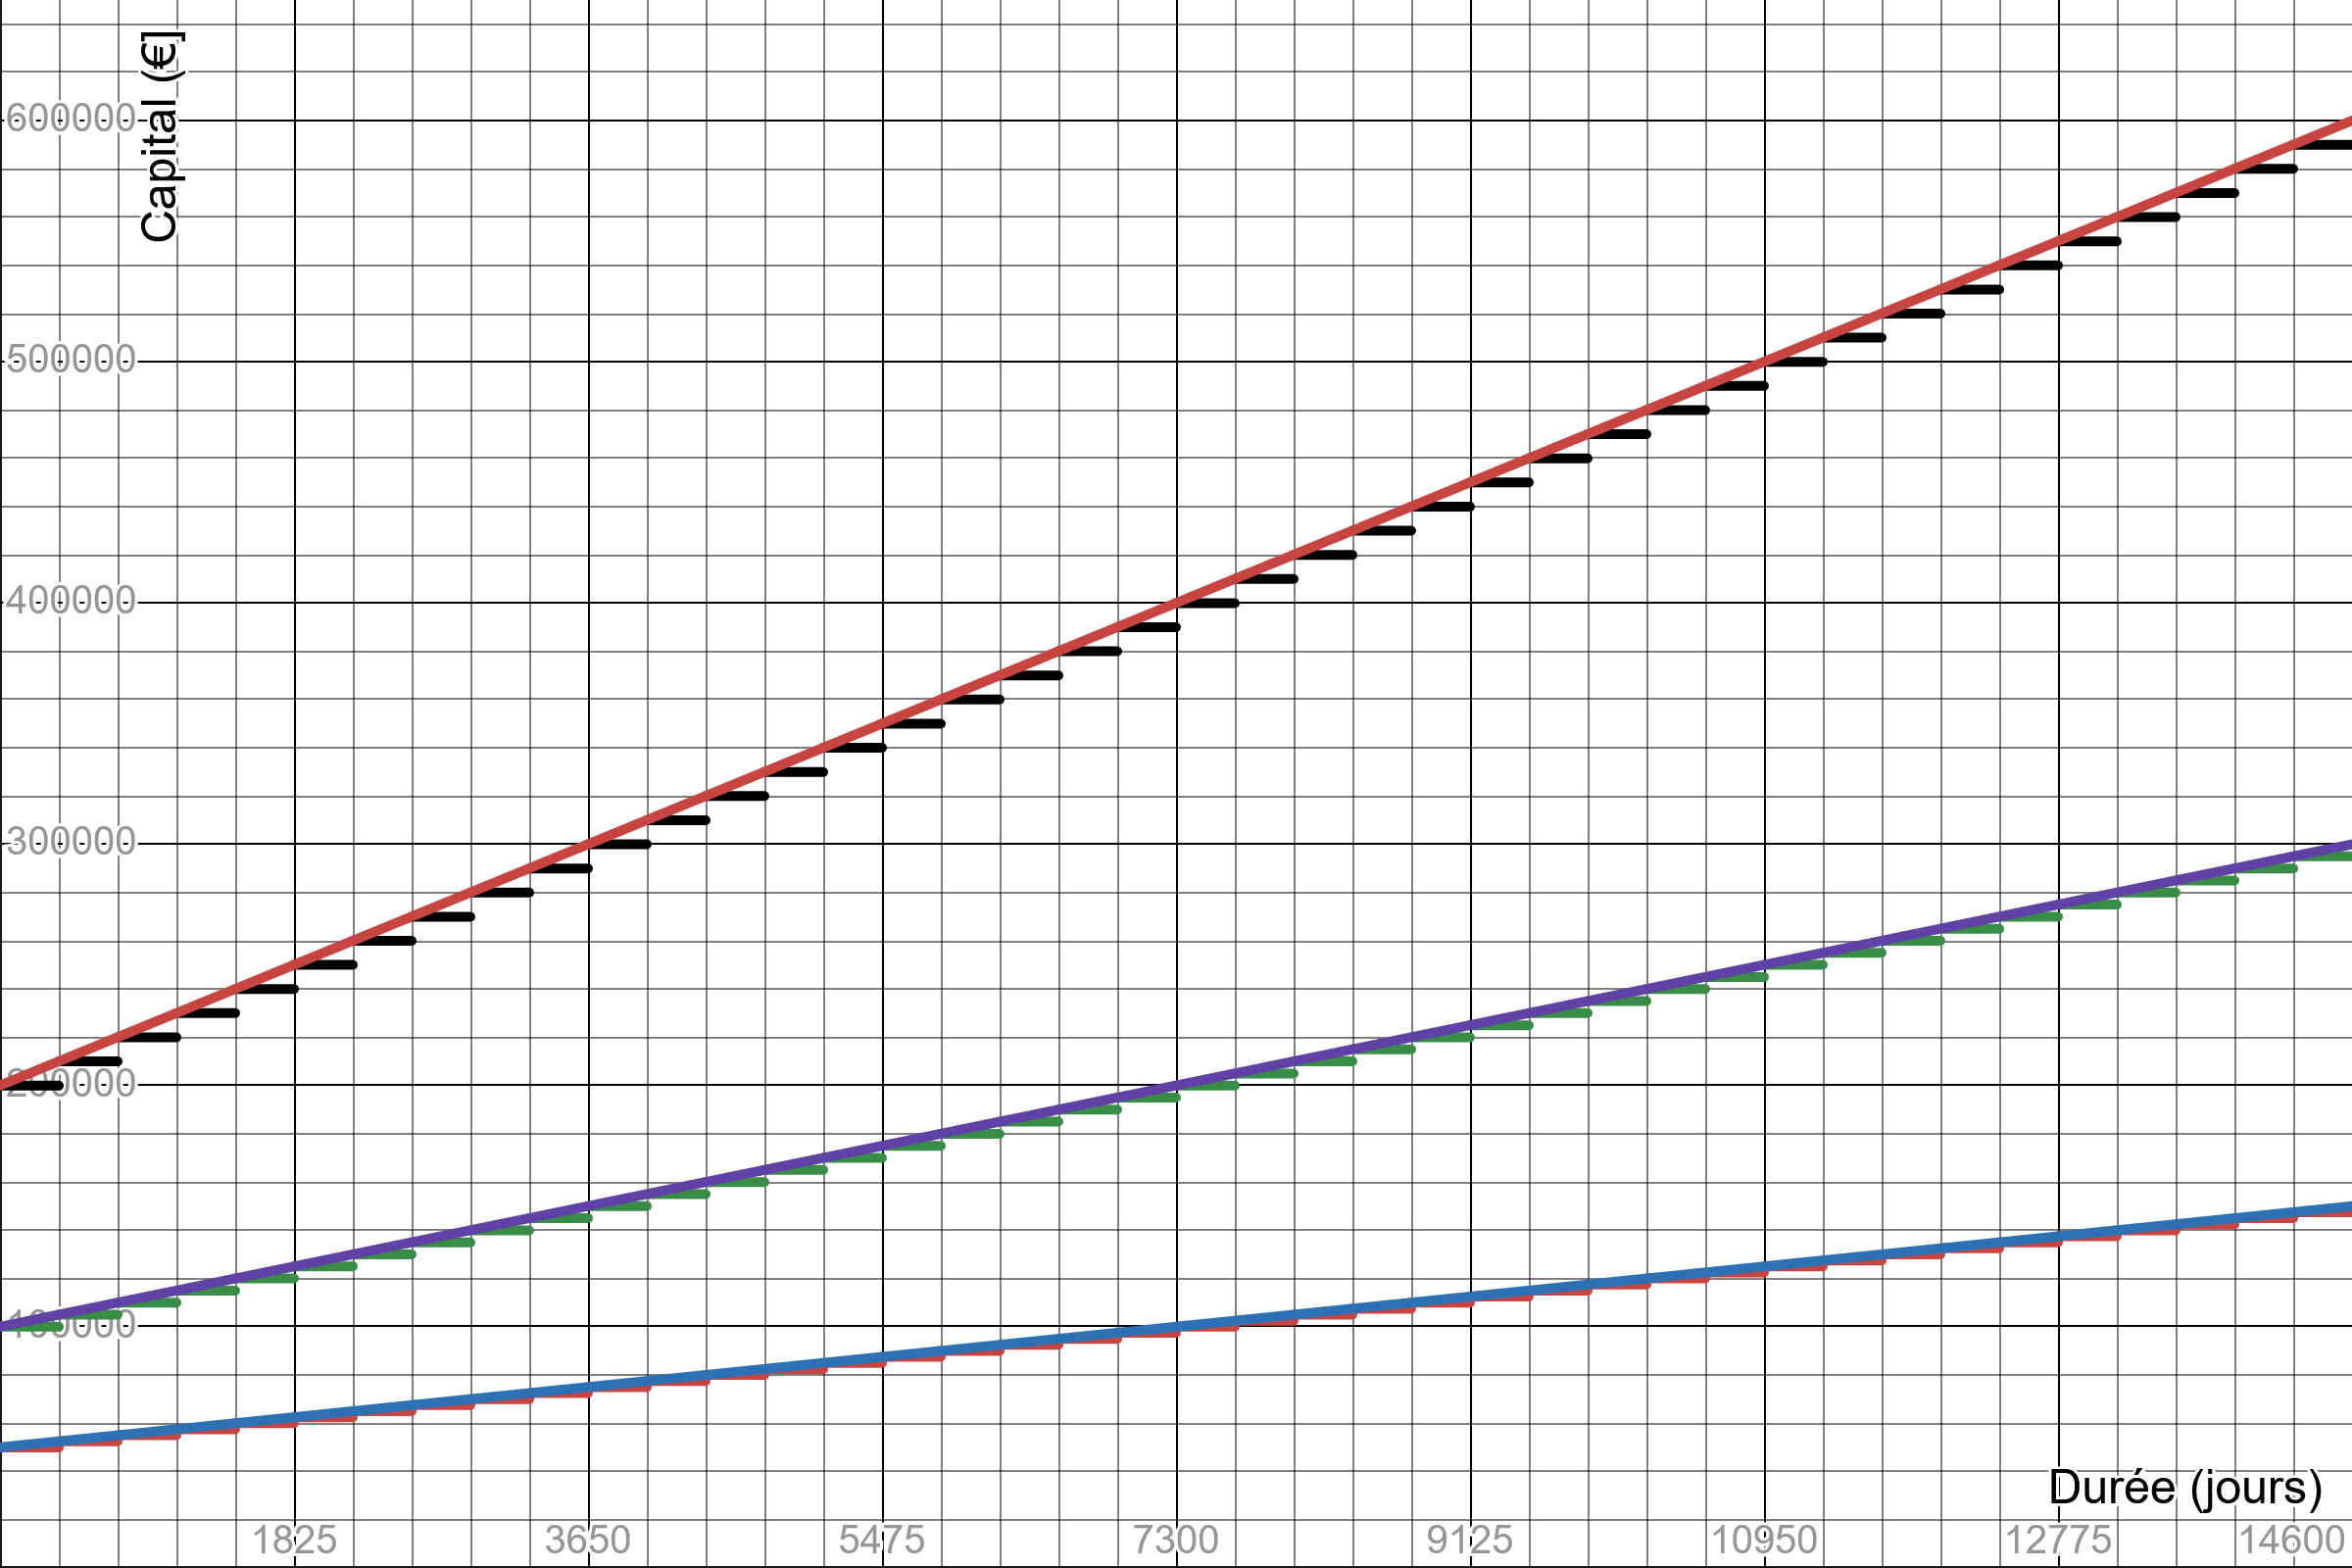
\includegraphics[width=\textwidth]{interets_simples.png}
        \caption{Comparaison de la capitalisation quotidienne et annuelle des intérêts simples.}
        \label{fig:interets_simples}
    \end{figure}

    \item Le capital final est lu graphiquement sur la figure \ref{fig:lecture_graphique_interets_simples}:
        \begin{align*}
            \begin{array}{rcl}
                50\,000\,\text{€}  & \xrightarrow{\text{10 ans}} & 75\,000\,\text{€} \\
                100\,000\,\text{€} & \xrightarrow{\text{10 ans}} & 150\,000\,\text{€} \\
                200\,000\,\text{€} & \xrightarrow{\text{10 ans}} & 300\,000\,\text{€} \\
                50\,000\,\text{€}  & \xrightarrow{\text{20 ans}} & 100\,000\,\text{€} \\
                100\,000\,\text{€} & \xrightarrow{\text{20 ans}} & 200\,000\,\text{€} \\
                200\,000\,\text{€} & \xrightarrow{\text{20 ans}} & 400\,000\,\text{€} \\
                50\,000\,\text{€}  & \xrightarrow{\text{30 ans}} & 125\,000\,\text{€} \\
                100\,000\,\text{€} & \xrightarrow{\text{30 ans}} & 250\,000\,\text{€} \\
                200\,000\,\text{€} & \xrightarrow{\text{30 ans}} & 500\,000\,\text{€}
            \end{array}
            \qquad
            \begin{array}{rrcl}
                10 \text{ ans :} & \displaystyle \frac{75\,000}{50\,000}  & = \displaystyle \frac{150\,000}{100\,000} & = \displaystyle \frac{300\,000}{200\,000} = 1,5 \\[1em]
                20 \text{ ans :} & \displaystyle \frac{100\,000}{50\,000} & = \displaystyle \frac{200\,000}{100\,000} & = \displaystyle \frac{400\,000}{200\,000} = 2 \\[1em]
                30 \text{ ans :} & \displaystyle \frac{125\,000}{50\,000} & = \displaystyle \frac{250\,000}{100\,000} & = \displaystyle \frac{500\,000}{200\,000} = 2,5
            \end{array}
        \end{align*}

        \begin{itemize}
            \item Le capital initial est multiplié par 1,5 après 10 ans.
            \item Le capital initial est multiplié par 2 après 20 ans.
            \item Le capital initial est multiplié par 2,5 après 30 ans.
        \end{itemize}
    
        \begin{figure}[h!]
            \centering
            \makebox[\textwidth][c]{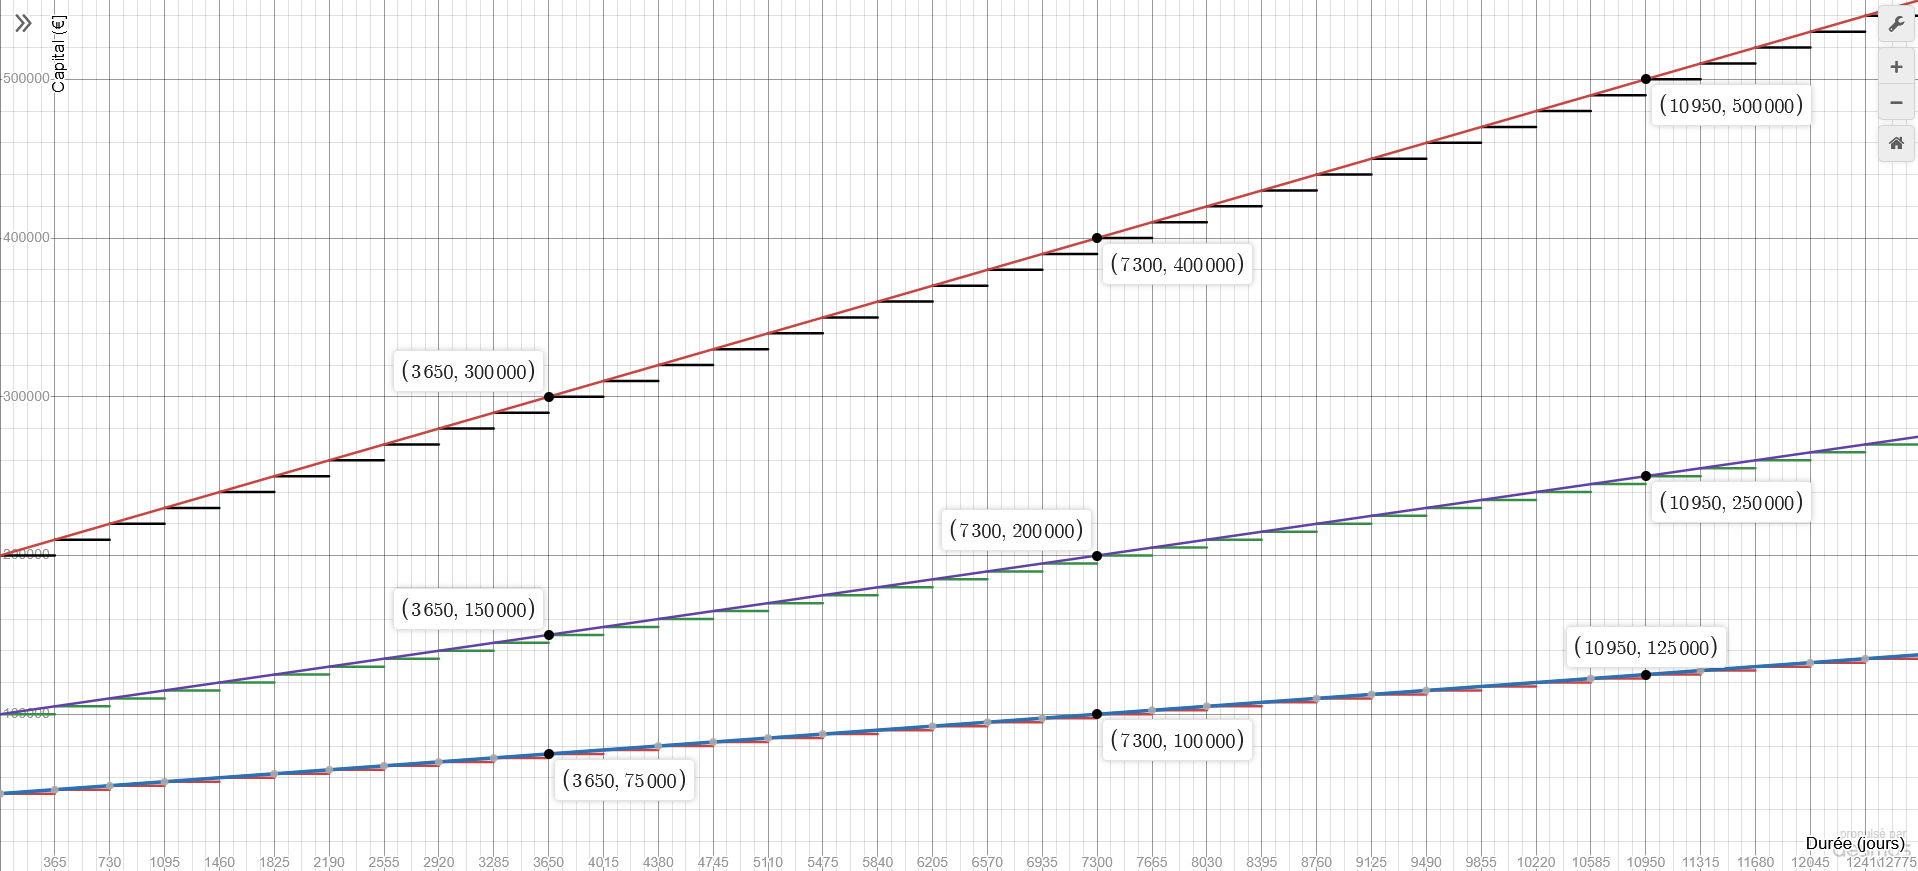
\includegraphics[width=1.35\textwidth]{lecture_graphique_interets_simples.png}}
            \caption{Lecture graphique du capital obtenu après 10, 20 et 30 ans d'investissement.}
            \label{fig:lecture_graphique_interets_simples}
        \end{figure}

        % Exprimer le coefficient multiplicateur du capital initial en fonction de la durée d’investissement et du taux périodique.
        \item Le coefficient multiplicateur du capital initial, noté \( k(t) \), représente le facteur par lequel le capital initial est multiplié pour obtenir le capital final après une certaine durée d'investissement \( t \), avec un taux périodique \( r_q \) (taux d'intérêt par période). Ainsi, le coefficient multiplicateur \( k(t) \) est le rapport entre le capital final \( C(t) \) et le capital initial \( C_0 \) :
        \[
        k(t) = \frac{C(t)}{C_0} = \frac{C_0 \left( 1 + r_q \cdot t \right)}{C_0} = 1 + r_q \cdot t = \boxed{1 + r_q \cdot t}
        \]

        Vérification :
        \begin{itemize}
            \item Pour 10 ans : $k(10) = 1 + 0,05 \times 10 = 1 + 0,5 = \boxed{1,5}$
            \item Pour 20 ans : $k(20) = 1 + 0,05 \times 20 = 1 + 1 = \boxed{2}$
            \item Pour 30 ans : $k(30) = 1 + 0,05 \times 30 = 1 + 2,5 = \boxed{2,5}$
        \end{itemize}

    
\end{enumerate}


\section{Prochaine étape}  
Développer un programme de simulation permettant de modéliser l'évolution du capital en fonction du montant investi, du taux de rendement, de la fréquence de capitalisation des intérêts et de la durée d'investissement. Le programme devra également calculer et afficher le taux d'intérêt effectif.  

\end{document}
